\chapter{The Cauchy-Kowalevski Theorem} \label{invariant}

Now that we have developed all the necessary tools, let us assume we have any Cauchy problem. As we showed in section \ref{pb}, it can be rewritten in the form:
$$
\begin{cases}
F(x,t, D^\alpha_x D^j_t u)=0 & |\alpha | +j \leq k\\
D^j_t u (x,0)= \phi_j(x) & \text{for }j<k 
\end{cases}
$$
Consequently, we will only deal with this last case, where the conditions are assigned on $\Gamma_0=\{ t=0 \}$.

The fundamental assumption of this chapter is that the data ($F$ and $\phi_j$) are analytic in a neighborhood of the origin, a property that we will use to show the existence of a unique \textbf{analytic solution}, still in a neighborhood of the origin.

However, to guarantee existence, we are forced to make some assumptions about the structure of the equation. 
Considering what has been said in the previous chapter, especially regarding theorem \ref{teoescar}, intuition suggests that it might be a good idea to consider the surface $\Gamma_0$ to be \textbf{non-characteristic}. 
This property allows us to rewrite the equation again in an even simpler form, namely:
\begin{equation}\label{pbnorm}
\begin{cases}
D_{t}^k u = G(x,t, D^\alpha_x D^j_t u) & |\alpha |+ j \leq k, \, j<k \\ 
D_t^ju = \phi_j & \text{ on } \Gamma_0, \, j<k
\end{cases} \\ 
\end{equation}
This idea will allow us to prove the TCK.
\begin{namedtheorem}[Cauchy-Kowalevski Theorem]
\hpth{
\text{Problem \eqref{pbnorm}}\\
G, \, \phi_j \text{ analytic in a neighborhood of the origin}
}
{\exists ! \; u \text{ analytic solution in a neighborhood of the origin}}
\end{namedtheorem}


After keeping as general a view as possible, we want to understand how to prove the result we have in mind. The approach we will follow will be "in reverse," progressively generalizing the results. Indeed, we will start from the least general case until we reach that of an equation in normal form, effectively following the chronological order of the results.


\newpage
\section{ODEs}

First, let us tackle a theorem very similar to the TCK, which deals with the case of a system of ODEs in normal form. 
We will start by stating the theorem.

\begin{theorem}\label{teoedo}
\hpth{
A \subseteq \mathbb{C}, \, B\subseteq \mathbb{C}^n \text{ open }\\
\Omega \subseteq A \text{ open connected}\\
f:A\times B\rightarrow\mathbb{C}^n \text{ holomorphic}\\
\text{Pb: }
\begin{cases}
y' = f(x,y) \quad \forall x \in \Omega \\ 
y(x_0)=y_0
\end{cases}\\
}
{
\text{locally, there exists a unique holomorphic solution}
}
\end{theorem}

\begin{remark}
This does not exclude the possibility of finding other non-analytic solutions.
\end{remark}

This result was the first application of the theory of holomorphic functions in combination with the method of majorants, which, as we already know, was proposed by Cauchy in the first half of the nineteenth century. 
We do not provide the full proof because it uses a different majorant from the one we introduced in section \ref{powerseries} (i.e., the one we will use to prove the TCK). 
In any case, it can be found in \cite{Delf}, and the structure of the reasoning is the same as that of theorem \ref{teoquasilin}.

Although we do not address the issue of existence in detail, it is worthwhile to discuss exhaustively the problem of \textbf{uniqueness} of analytic (or holomorphic) solutions. An analytic function is uniquely determined by all its derivatives at a point, which, in this case, are known due to the analyticity of the function $f$.
We completely conclude the discussion by also addressing the situation of a PDE: here too, assuming the data are analytic, it is possible to know all the partial derivatives of the function, thanks to the fact that the surface on which the conditions are assigned is assumed to be non-characteristic.

Since this result has been demonstrated by constructing a majorant for the solution $y$, it is possible to obtain an estimate of its radius of convergence by using theorem \ref{theomaj}.

\begin{theorem}
\hpthml{
\text{Assumptions of theorem \ref{teoedo}}\\
\exists \, \overline{B_a(x_0)}\subseteq A,\,\overline{B_b(y_0)} \subseteq B\\
M=\max_{B_a(x_0),\, B_b(y_0)}|f|
}{
\text{The solution has radius at least } \widetilde{r}= a\left[ 1-\exp\left( -\frac{b}{aM(n+1)}\right) \right] 
}
\end{theorem}

\begin{remark}
It is interesting to note what happens when $B=\mathbb{C}^n$.
\end{remark}


\newpage
\section{Quasi-linear PDEs}

Now it is time to address the cornerstone of the entire reasoning about PDEs, namely the theorem that shows the existence, and thus also the uniqueness, of an analytic solution to a quasi-linear system of PDEs in normal form.

\begin{theorem}\label{teoquasilin}
\hpth{
A_i, \, B \text{ analytic in a neighborhood of the origin }\\
\text{Pb: }
\begin{cases}
D_t \, y = \sum\limits_{i=1}^{n-1} A_i(x,y)D_{x_i}y+B(x,y) \; \\ 
y=0 \quad \text{ on } \Gamma_0
\end{cases}
\\
}{
\exists ! \; y(x,t): \mathbb{R}^n \rightarrow \mathbb{R}^m
\text{ analytic solution in a neighborhood of the origin}
}
\end{theorem}

\begin{remark}
This theorem can easily be modified by replacing analyticity with \textbf{holomorphy}, in order to obtain a statement similar to the case of ODEs, as the extension is immediate since no particular assumption distinguishes the real case from the complex one in the proof.
\end{remark}

\begin{proof}
First of all, let us denote by $a^i_{ml}$ the components of $A_i$ and $b_m$ those of $B$, while the coefficients of the series are respectively $(a^i_{ml})_\gamma$ and $(b_m)_\gamma$. Now let us proceed step by step.
\begin{enumerate}
\item Considering component by component, we assume $y_h = \sum c^h_{\alpha j} x^\alpha t^j$ with ${h=1,\ldots, m}$.
\item The Cauchy condition tells us that $c^h_{\alpha 0}=0$.
\item By inserting the series for $y,\, A_i,\, B$ into the equation and using theorems \ref{composition}, \ref{derivative} and \ref{product}, we obtain for each row $h$ the equation:
$$\sum\limits_{\alpha, \, j} (j+1)c^h_{\alpha (j+1)}\, x^\alpha t^j = \sum\limits_{\alpha,\, j} P_{\alpha j}\left((c^h_{\alpha l})_{l\leq j},(a^i_{ml})_\gamma, (b_m)_\gamma\right) \, x^\alpha t^j$$
where the polynomials $P_{\alpha j}$ are naturally non-negative coefficients.
\item Thanks to this operation, we derive a recursive formula for the coefficients:
$$ c^h_{\alpha (j+1)}= (j+1)^{-1} P_{\alpha j}\left((c^h_{\alpha l})_{l\leq j},(a^i_{ml})_\gamma, (b_m)_\gamma\right),$$
which allows us to conclude that $c^h_{\alpha j} = Q_{\alpha j}\left((a^i_{ml})_\gamma, (b_m)_\gamma\right)$ where $Q_{\alpha j}$ are always polynomials with non-negative coefficients, the form of which does not depend on $A_i$ and $B$. Thus, we can also say that it is always possible to construct a power series that satisfies the equation. We are left to understand whether it converges with a positive radius.
\newpage
\item Now suppose we have another problem with the same structure defined by the functions $\widetilde{A}_i $ and $\widetilde{B}$ and we know a local analytic solution $\widetilde{y}$. We want to show that $$\widetilde{A}_i \gg A_i, \, \widetilde{B} \gg B \implies \widetilde{y} \gg y.$$
Considering that for both problems the same considerations hold up to point 4 (the polynomials $Q_{\alpha j}$ are the same!), we can write the following chain of inequalities:
\begin{align*}
\left|c^h_{\alpha j}\right| &= \left|Q_{\alpha j}\left((a^i_{ml})_\gamma, (b_m)_\gamma\right)\right|\\
&\leq Q_{\alpha j}\left(\left|(a^i_{ml})_\gamma\right|, \left|(b_m)_\gamma\right|\right) 
& \text{non-negative coeff.}\\
&\leq Q_{\alpha j}\left((\widetilde{a}^i_{ml})_\gamma, (\widetilde{b}_m)_\gamma\right) = \widetilde{c}^h_{\alpha j}
& \widetilde{A}_i \gg A_i, \, \widetilde{B} \gg B
\end{align*}
\item The last step consists in choosing $\widetilde{A}_i, \, \widetilde{B}$, in such a way as to explicitly calculate $\widetilde{y}$ and show that it is analytic. Given our knowledge about the power series that come from theorem \ref{constmaj}, we know how to construct an upper bound for $A_i$ and $B$. Thus, we select two constants $C$ and $r$ such that 
$$\frac{Cr}{r-(x_1+\ldots +x_{n-1})-(y_1+\ldots +y_m)}=\mathcal{M}_{Cr}(x,y) \gg A_i(x,y),\, B(x,y)$$
and that satisfy the inequalities \eqref{r} and \eqref{C}. We then define the problem
\begin{equation*}
\begin{cases}
D_t \, \widetilde{y}_h = \mathcal{M}_{Cr} (x,y) \left[\sum\limits_{i,\, j} D_{x_j}\widetilde{y}_i+1 \right] \\ 
\widetilde{y_h}=0 \quad \text{ on } \Gamma_0
\end{cases}
\end{equation*}
where $h=1,\ldots, m$. At this point it is possible to show, using the method of characteristics for quasi-linear first-order equations (paragraph \ref{metodocar}), that it has the solution
\begin{equation}\label{maggiorante}
\widetilde{y}_h(x,t)=u(x_1+\cdots +x_{n-1},\,t) \quad \forall h
\end{equation}
where
\begin{equation}\label{sol}
u(s,t)=\frac{r-s-\sqrt{(r-s)^2-2tCrmn}}{mn},
\end{equation}
which is clearly analytic in a neighborhood of the origin. See \cite[cap.1]{Folland} for the complete unfolding of the calculation.
\item We conclude by observing an interesting fact: there is nothing specific that guarantees that the solution found continues to ensure the upper bound. In fact, it is important to verify that $\widetilde{y}$ satisfies the inequality $|(x,\widetilde{y}(x,t))|< r$ (so that $\mathcal{M}_{Cr}$ is indeed a power series). For more details, see proposition \ref{prop}.
\end{enumerate}
\end{proof}


\newpage
As in the case of the system of ODEs, if we utilize theorem \ref{theomaj}, we can estimate the radius of convergence by studying the radius of the dominating solution in \eqref{maggiorante}. 

\begin{theorem}\label{stimaraggio}
The solution of Theorem \ref{teoquasilin} converges with a radius of at least
$$\widetilde{r} = \dfrac{1}{n-1}\, \dfrac{r}{8Cmn} \text{ with } C \geq \frac{1}{2}$$
\end{theorem}
\begin{remark}
$n \geq 2$ for the system to be truly in partial derivatives. 
\end{remark}
\begin{remark}
It is interesting to focus on the behavior with respect to $r$, knowing that:
\begin{align}\label{r}
r <& \min \{ \textit{radii of convergence of the coefficients } a^i_{ml}, \, b_m\} \\ 
\label{C}
C \geq & \max \begin{Bmatrix}
\max\limits_{i,m,l,\alpha } \left| (a^i_{ml})_\alpha \, r^{|\alpha |}\right|\\
\max\limits_{m,\alpha} \left|(b_m)_\alpha \, r^{|\alpha |}\right|
\end{Bmatrix}
\end{align}
\end{remark}

\begin{proof}
Let us fix $r$ and $C$ as above, and furthermore assume that $C \geq 1/2$ (we can do this without any problem). 
Initially, we focus on the function in \eqref{sol}, which is analytic in a neighborhood of the origin, particularly in the set 
$$A = \left\{ (s,t) \in \mathbb{R}^2 : t<\frac{(r-s)^2}{2Crmn} \right\} .$$
That is, it can be expanded in a power series in $B_l(0)$ with $0<l<d=\text{dist}(0, \partial A)$.
\begin{center}
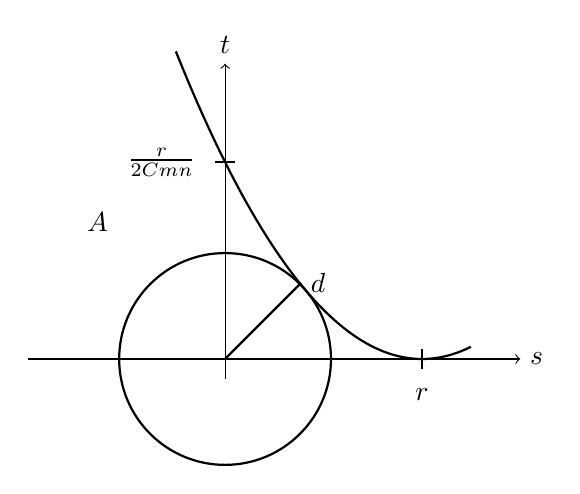
\begin{tikzpicture}[scale=2.5]
    % Draw the circle centered at (0,0) with radius 0.538
    \draw[thick,black] (0,0) circle[radius=0.538];
    
    % Draw the parabola y = (1-x)^2
    \draw[thick,black,domain=-0.25:1.25,samples=100] 
        plot ({\x}, {(1-\x)^2});
    
    \node[black,anchor=south west] at (-0.75, 0.60) {$A$};
    
    % Draw the axes
    \draw[->] (-1,0) -- (1.5,0) node[right] {$s$};
    \draw[->] (0,-0.1) -- (0,1.5) node[above] {$t$};
    
    % Draw the segment from (0,0) to (sqrt{0.538/2}, sqrt{0.538/2})
    \draw[thick,black] (0,0) -- (sqrt{0.538/1.9},sqrt{0.538/1.9});
    \node at (sqrt{0.538/1.9},sqrt{0.538/1.9}) [right] {$d$};
    
    % Draw the ticks
    \draw[thick] (1, 0.05) -- (1, -0.05); % Tick at (1, 0)
    \node at (1, -0.1) [below] {$r$};    % Label for (1, 0)
    
    \draw[thick] (-0.05, 1) -- (0.05, 1); % Tick at (0, 1)
    \node at (-0.1, 1) [left] {$\frac{r}{2Cmn}$}; % Label for (0, 1)
    
\end{tikzpicture}
\end{center}
Choosing $l_1 = (n-1)\,\widetilde{r}$, it can be shown that, for $C>1/8$, we indeed have that $l_1<d$. The goal would therefore be to verify that $$\sqrt{l_1^2-s^2} < \frac{(r-s)^2}{2Crmn}$$ for every $|s|<l_1$, but this is implied by 
\begin{equation} \label{l1}
l_1 < \frac{(r-l_1)^2}{2Crmn}\; ,
\end{equation}
an inequality that holds true if and only if $C > 1/(4mn) \leq 1/8$.

Now, we will generalize this for the function $\widetilde{y}_h$ in \ref{maggiorante} with $h$ fixed. It is analytic in the region 
$$A = \left\{ (x,t) \in \mathbb{R}^n : t<\frac{(r-(x_1+\ldots +x_{n-1}))^2}{2Crmn} \right\} .$$
The structure of the problem remains the same, so, naturally, the definition of $d$ remains unchanged. The only aspect we need to take care of is that, in this situation, it will be necessary to choose $l_2 =\widetilde{r}$. 
Thus, we want to show that $$\mathcal{L}=\sqrt{l_2^2-(x_1^2+\ldots +x_{n-1}^2)} < \frac{(r-(x_1+\ldots +x_{n-1}))^2}{2Crmn}=\mathcal{R}$$
when $|x|=|(x_1,\ldots ,x_{n-1})|< l_2$. But this is implied by the inequality \ref{l1}, which we know to be true. We will prove it in two steps.
\begin{itemize}
\item It holds that $\mathcal{L}^2< l_2^2 \leq l_1^2$ for $|x|< l_2$.
\item It holds that $$\left(\frac{(r-l_1)^2}{2Crmn}\right)^2 \leq \min \left\{ \mathcal{R}^2 : |x|\leq l_2 \right\}< \mathcal{R}^2 \, \text{ for } \, |x|< l_2.$$
This is shown knowing that $$\max \left\{ x_1+\ldots +x_{n-1} : |x|\leq l_2\right\}= (n-1)\frac{l_2}{\sqrt{n-1}}\leq l_1$$ and showing that $r-(x_1+\ldots +x_{n-1})>0$ for $|x|\leq l_2$ with the triangle inequality.
\qedhere
\end{itemize}
\end{proof}

\noindent\rule[0.5ex]{\linewidth}{0.2pt}

A careful reader will surely wonder about the reason behind choosing a constant $C\geq 1/2$. Well, this issue arises from what was left open in the proof of Theorem \ref{teoquasilin}, namely the fact that the solution $\widetilde{y}$ is indeed dominating only if $|(x,\widetilde{y}(x,t))|< r$. This property is precisely guaranteed in a ball of radius $\widetilde{r}$. Let us see this with a proposition that, in addition to clarifying, completes the logical framework of the proofs.
\begin{namedtheorem}[Proposition]\label{prop}
The domination of $\widetilde{y}$ holds in $B_{\widetilde{r}}(0)$, i.e.
$$|(x,t)|<\widetilde{r} \implies |(x,\widetilde{y}(x,t))|=x_1^2 + \ldots + x_{n-1}^2 + m \, u^2(x_1 + \ldots + x_{n-1},t) < r^2$$
\end{namedtheorem}
\begin{proof}
For simplicity, we demonstrate that $$|(s,t)|< l=(n-1)\,\widetilde{r} \implies s^2 + m \, u^2(s,t) < r^2.$$ The generalization is trivial if we take inspiration from the proof of Theorem \ref{stimaraggio}. 
\newpage
Considering that $|t|,|s|<l<r$ and that $s^2+t^2<l^2=r/(8Cmn)$, we write the following chain of inequalities.
\begin{align*}
& s^2 + m \left[ \frac{r-s-\sqrt{(r-s)^2-2tCrmn}}{mn} \right]^2\\ 
&\leq s^2 + \frac{1}{mn^2} \left[ (r-s)^2 + |(r-s)^2-2tCrmn| \right] 
&\begin{system}
\left|s\right| < r \Rightarrow r-s > 0\\
 \sqrt{(r-s)^2 - 2t Cr mn} > 0 
\end{system}\\
&\leq s^2 + \frac{2}{mn^2} (r-s)^2 + \frac{2|t|Crmn}{mn^2} \\ 
&\leq l^2 + \frac{2}{mn^2} \left( r^2 + l^2 + 2rl \right) + \frac{2lCrmn}{mn^2} 
&\begin{system}
\left|s\right| < l \Rightarrow (r-s)^2 < (r+l)^2\\
\left|t\right| < l
\end{system}\\
&= \left( \frac{r}{8Cmn} \right)^2 + \frac{2r^2}{mn^2} \left[ 1+\frac{1}{(8Cmn)^2} + \frac{1}{4Cmn} + \frac{1}{8} \right] \\ 
&< r^2 \underbrace{\frac{2}{mn^2} \left[ \frac{r}{8} + \frac{1}{(8C)^2 mn^2} + \frac{r}{(8Cmn)} + \frac{r}{4Cmn} + \frac{1}{8} \right]}_{<1} < r^2 \\ 
\end{align*}
In particular, the last statement holds because
\begin{align*}
n \geq 2 \Rightarrow \frac{2}{mn^2} \left(\ldots\right) 
&\leq \frac{1}{2} \left(\frac{9}{8} + \frac{2}{(8C)^2} + \frac{1}{8C}\right) \\ 
& \leq \frac{3}{16} \left(3 + \frac{1}{C}\right) < 1 & \Leftarrow C \geq \frac{1}{2} 
\end{align*}
\end{proof}



\newpage
\section{EDP in Normal Form}
Now we will utilize the results from the previous section to generalize that result to the case of an equation in normal form. To do this, it is sufficient to state and prove the following theorem.
\begin{theorem}\label{teonorm}
The following two problems are equivalent
\begin{align*}
\text{non-linear: }&
\begin{cases}
D_{t}^k u = G(x,t, D^\alpha_x D^j_t u) & |\alpha |+ j \leq k, \, j<k \\ 
D_t^ju = \phi_j & \text{ on } \Gamma_0, \, j<k 
\end{cases} \\ 
\text{quasi-linear: }&
\begin{cases}
D_t \, y = \sum\limits_{i=1}^{n-1} A_i(x,y)D_{x_i}y+B(x,y) \; \\ 
y=0 \quad \text{ on } \Gamma_0 
\end{cases}
\end{align*}
\end{theorem}

\begin{proof}
The reasoning is divided into three steps:
\begin{enumerate}
\item We construct the system such that $y_{\alpha j}= D^\alpha_x D^j_t u$. \\ 
Then, the matrices $A_i$ and $B$ can be obtained from the expressions
\begin{align*}
D_t y_{\alpha j} =& y_{\alpha (j+1)} & |\alpha| + j < k \\ 
D_t y_{\alpha j} =& D_{x_l} y_{(\alpha-e_l)(j+1)} & |\alpha| + j = k, \; j < k \\ 
D_t y_{0k} =& D_tG + \sum_{|\alpha|+j < k} D_{y_{\alpha j}}G y_{\alpha (j+1)} \\ 
& + \sum_{|\alpha|+j = k, \; j < k} D_{y_{\alpha j}} G D_{x_l} y_{(\alpha-e_l)(j+1)}
\end{align*}
where $l(\alpha)=\min\{ l:\alpha_l\neq 0 \}$, and the Cauchy data will be
\begin{align*}
y_{\alpha j}(x, 0) = & D_x^{\alpha} \phi_j(x) & j < k \\ 
y_{0k}(x, 0) = & G\left( x, 0, D_x^{\alpha} \phi_j(x) \right) & \lvert \alpha \rvert + j \leq k, \; j < k 
\end{align*}
\item We remove the conditions $\phi$, redefining $y(x,t)\leftarrow y(x,t)-\phi (x)$.
\item We eliminate the dependence on $t$, adding the variable $y^0=t$, together with the equation $D_t y^0=1$ and the data $y^0(x,0)=0$.
\end{enumerate}
We conclude by stating that, obviously, if $u$ is a solution of the problem in normal form, the $y_{\alpha j}$ will be solutions of the newly constructed problem. However, to demonstrate that $y_{(0,\ldots,0)}$ (solution of the latter) is also a solution of the problem in normal form, various calculations are necessary, which can be found in detail in \cite[cap.1]{Folland}.
\end{proof}

\begin{remark}
There are three aspects, which also emerge from the proof, that are worth briefly reflecting upon:
\begin{itemize}
\item Bringing together the considerations made at the beginning of the chapter and the theorems \ref{teoquasilin} and \ref{teonorm}, the TCK follows immediately;
\item The estimate of the radius of convergence continues to hold;
\item This equivalence theorem can be readily generalized to the case of a system in normal form.
\end{itemize}
\end{remark}
